\documentclass{cacthesis}
\usepackage[ruled,vlined]{algorithm2e}
\usepackage{tabularx}

\newcounter{protocol}
\newenvironment{protocol}[1]
  {\par\addvspace{\topsep}
   \noindent
   \tabularx{\linewidth}{@{} X @{}}
    \hline
    \refstepcounter{protocol}\textbf{Protocol \theprotocol} #1 \\
    \hline}
  { \\
    \hline
   \endtabularx
   \par\addvspace{\topsep}}

\newcommand{\sbline}{\\[.5\normalbaselineskip]}% small blank line

\begin{document}

	\frontmatter
	
	%%%%%%%%%%%%%
	%% Title page
	%%%%%%%%%%%%%
	\title{Fair Exchange Protocol over Bitcoin}
	\author{Leandro Rometsch}
	\date{October 19, 2020}
	\subject{Bachelor Thesis}
	
	\publishers{
		\small
		\begin{tabular}{r l}
			Supervisors: Benjamin Schlosser, \\ Prof. Sebastian Faust, Ph.D.
		\end{tabular}
	}
	\maketitle
	
	\tableofcontents
	
	\mainmatter
	
	\chapter{Introduction}
        %Sum up the basics of a data exchange protocol. Talk about the possibilities of smart contracts, how they can realize data exchange protocols, and why Bitcoin based smart contracts might be a good alternative to Ethereum based ones. 
        
        We describe an exchange scenario, where a buyer $B$ is willing to spend money in exchange for a product offered by seller $S$. $B$ expects the product to be in a particular condition beforehand. In a traditional setting, where both parties and the product are physically available at one place, $B$ can check for himself before paying if the product he planned to buy is the way $B$ expected it to be. If the expectation is not met, $B$ will not pay for the product - if it is, the exchange can be completed with minimal risk because both parties can be held liable. Neither $B$ nor $S$ got any disadvantage. \\
        This procedure is not trivially transferable to a digital setting - especially if digital goods are being exchanged. Digital items can be copied indefinitely and are not directly limited by supply. We assume $B$ wants to buy a digital product $d$, e.g., a song or a movie, and still got a certain expectation beforehand - this expectation is met if the predicate $\sigma\left( d\right) =1$. The dilemma is the following: Either $S$ needs to reveal its digital commodity $d'$ first to let $B$ check if $\sigma\left( d'\right) =1$, or B needs to pay beforehand without being able to inspect $d'$. Without trust among the two parties, this is undoubtedly vulnerable to fraud, and trust is not an ideal requirement in a digital setting where liability is limited. There are no security cameras, witnesses, nor is police on hand. \\ 
        One way to solve this dilemma is to introduce a middleman, some kind of Trusted Third Party (TTP) to the exchange - similar to Certification Authorities that issue digital certificates. The TTP can independently verify if Bs expectation $\sigma$ is fulfilled and secure a fair exchange. Unfortunately, a dedicated middleman comes with significant drawbacks: A service like this is usually expensive, both parties need to agree on a specific one, and the availability is questionable. \\
        Cryptocurrencies offer huge potential here, with their smart contracts imitating the middleman. A smart contract enables the transfer of money conditionally. The buyer and the merchant do not need to trust a single entity anymore. The only construct to trust is the decentralized blockchain of the used cryptocurrency that evaluates a smart contract's conditions. The main difficulty here is that memory is financially limited on the blockchain via fees. The naive approach of letting a smart contract evaluate $\sigma\left( d'\right)$, s.t. $\sigma$ is the condition to execute the monetary transfer, is only feasible if $d'$ consists of a few bytes but practically fails for larger files due to high fees - especially because digital items are usually relatively inexpensive. Another point to consider is that everything on the blockchain is public. Therefore the naive approach is surely not advantageous for $S$. Using smart contracts that support the cheap and private exchange of larger files (as an alternative to expensive TTP) requires a different protocol design - there are good solutions out there, but more on this in the next section.   \\ 
        For a fair exchange protocol building on a particular cryptocurrency, an important aspect is the number of users the currency got. Choosing a cryptocurrency with a big user base increases the acceptance of the protocol. The most prominent technologies here are Bitcoin and Ethereum. They both offer two completely distinct approaches when it comes to the construction of smart contracts. Ethereum, on the one hand, offers a powerful virtual machine that enables the formulation of complex conditions and, therefore, powerful protocols via its statically-typed and object-oriented programming language. On the other hand, Bitcoin only supports basic payment transactions based on a simple stack-based scripting language. Usually, fair exchange protocols utilizing Bitcoin are less efficient or lack a high fairness guarantee. \\
        This thesis aims to analyze whether it is possible to construct an efficient and cheap fair exchange protocol on top of Bitcoin rather than most other protocols achieving these properties utilizing Ethereum. A solution is particularly interesting because it would make cheap fair exchange accessible for a broader market while potentially reducing the complexity on the blockchain itself.
        % Move this into the contribution section: Therefore, we will look into efficient Ethereum based protocols and investigate the possibility of transferring one to Bitcoin, making it accessible for a broader market.
        
        \section{Existing solutions}
        % Briefly write about the interesting fair exchange protocols I reviewed in the research phase. What is the most exciting aspect of them? What can we learn from them?
        All efficient approaches have in common that they use the blockchain as a trusted anchor and only utilize it when necessary to minimize fees. The computation done by the participating parties locally is usually much cheaper and, therefore, preferred against expensive computation done by the smart contract. \\
        The fair exchange protocols utilizing Bitcoin usually choose computationally demanding zero-knowledge proofs (\cite{zkcp}\cite{DELGADOSEGURA2020832}), mainly because of the limitations Bitcoins smart contracts have. Other approaches, primarily Ethereum based ones, try to avoid these computational burdens while simultaneously keeping the protocol participants' fees low. FairSwap \cite{10.1145/3243734.3243857}, for example, enables $B$ to prove misbehavior of a merchant afterward instead of checking $\sigma$ beforehand. Optimistic protocols like this one are advantageous because they usually only need to perform costly blockchain interaction if fraud is suspected, making the optimistic case very cheap. The cheap optimistic case is highly desirable, especially if there is no incentive for one of the parties to cheat. One way to remove any incentive, also concerning Denial of Service (DoS) attacks, is to introduce unavoidable penalties when misbehaving. \\
        One crucial part of every fair exchange protocol is how to design $\sigma$, or informally speaking, the data correctness proof s.t. $B$ can verify for itself that the product advertised by $S$ is the expected one. Different approaches do this either before or after the data exchange. Delagado et al. use a cut-and-choose technique in the first phase of their Bitcoin-based protocol [cite Delgado], which splits the file into many single but still meaningful chunks. E.g., if $B$ expects to buy a specific movie from $S$, the movie is split up its frames. A small subset of these frames is manageable for $B$ to verify beforehand, which gives (depending on the size of the subset) $B$ the confidence to proceed in the exchange. FairSwap does this the other way around by assuming a public fingerprint is available for every digital item being exchanged. After the actual file exchange, $B$ then computes the fingerprint on his own and compares it to the public one. If they do not match, $B$ can prove this to the protocol through the smart contract and get a refund.
        
        
        
        \section{Contribution}
        Understanding the current concept of fairness (and the problems relating to it). \\
        What is necessary to convert a script like FairSwap onto a potentially cheaper Bitcoin variant, and why it is challenging.
        FairSwap inspired fair exchange protocol that runs cheaper on Bitcoin Script.

        \section{Related Work}
        How Bitcoin evolved to Bitcoin Cash. What are the key differences between Bitcoin, Bitcoin Cash, and Ethereum in terms of smart contracts?.
    
    \chapter{Preliminaries}
        \section{Bitcoin}
        In 2008 Satoshi Nakamoto proposed the first practical decentralized peer-to-peer currency system (commonly known as "cryptocurrency"), named Bitcoin \cite{nakamoto2009bitcoin}. The premise of Bitcoin is a shared data structure maintained by a decentralized network of nodes. This data structure is made out of cryptographically chained blocks, the so-called blockchain, that miners continuously work on extending. One new block added to the blockchain allows for a certain amount of new payment transactions and simultaneously increases the integrity of the blocks before. Other cryptocurrencies might extend their blockchain differently. However, in Bitcoin's case, this \textit{proof-of-work} approach is used, such that the blockchain's integrity is guaranteed, as long as the honest nodes control more than half of the CPU power. For the computational burden the miners take, they are compensated with newly generated Bitcoins and transaction fees. The result is a self-sustaining system that is fully decentralized and trustable. From a high level, Bitcoin can be considered as an emulated trusted bank without a single entity controlling it.  The trust in Bitcoin is exceptionally high because there were practically no successful attacks yet. This fact is essential for the acceptability of a decentralized currency system because no central institution could be held liable. The users' trust rests in the \textit{proof-of-work} consensus protocol that secures the validity of transactions and prevents double-spending. \\
        It is notable that Bitcoins blockchain only stores transactions of Bitcoins (and some metadata to secure the blockchain) and only implicitly stores the user's balances. The name Bitcoin might be misleading here because there are no actual coins, only a traceable path of transactions that originate from a miner's reward. The amount of Bitcoin one person owns can be calculated by looking at every transaction this person received but did not spend jet. If a person wants to perform a Bitcoin transaction, it needs access to at least one key pair containing one public key and one private key. The public key is essentially the person's address, which enables him/her to receive Bitcoins. The private key is needed to send Bitcoins to other users' public keys. Because everybody can create arbitrary key-pairs without providing any personal information, Bitcoin provides some anonymity for its users. \\
        The introduction of Bitcoin, especially the blockchain concept, kickstarted many other cryptocurrencies and blockchain-based applications. Still, Bitcoin is the most widely accepted cryptocurrency and remains the largest by market capitalization\footnote{Source: \url{https://coinmarketcap.com/} (14.12.2020)} - followed by Ethereum and XRP.

        \subsection{BTC Transactions}
        Technically there are no Bitcoins, only transactions of a particular Bitcoin value that are either spent or unspent. Each new transaction needs at least one input transaction. The sum of the value of all input transactions determines the value of the new transaction. Once a transaction is published in a new block on the blockchain, its input transaction(s) are considered spent. A new transaction itself is unspent until it is again used for some other valid transaction as input. Only unspent transactions can be used as an input transaction. If one of the input transactions is already spent, the new transaction is recognized as invalid and rejected by the network. \\
        The other two essential parts of every Bitcoin transaction are the out script and the witness. The out script contains the condition(s) that need to be fulfilled by somebody that wants to spend the transaction. The witness is the values that are given as input to the out script. Consequently, the out script is the lock of a transaction, and the witness is the key. Note that the witness inside a transaction is not related to its own out script - it is needed to unlock the out script of the input transaction(s). Therefore, if the user knows the correct values to fulfill the out script of an unspent transaction, it practically owns the particular Bitcoins. Take \ref{fig:tx1} as an example. The out script is written in Bitcoin's scripting language (see next section) and is usually utilized to perform standard payments to a single Bitcoin address (P2PKH). More complex out scripts are possible that enable payments under a wide variety of conditions, e.g., timelocks or the signatures of multiple users.
        \begin{figure}
          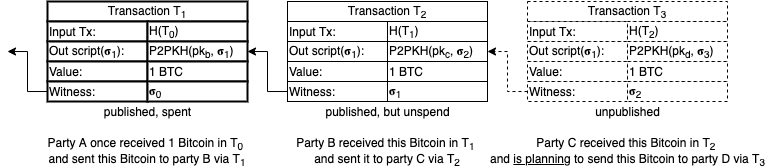
\includegraphics[width=\linewidth]{images/basic_transaction_figure.png}
          \caption{Example of a Bitcoin transaction trace.}
          \label{fig:tx1}
        \end{figure}
        \\ For an efficient transaction validity evaluation, each node stores, in addition to the blockchain (or parts of it), two transaction pools locally: The pending transaction pool and the unspent transaction pool. Pending transactions are valid transactions requested for execution but are not included in a blockchain block yet. If a node receives a new valid transaction from a user, the node puts it into its pending transaction pool and forwards it to all connected peers. Once a new block is added to the blockchain, a node deletes all transactions the new block contains from its pending transaction pool and updates its unspent transaction pool. Suppose a node wants to evaluate the validity of the input transactions of a new transaction. In that case, it checks if all input transactions are available in the unspent transaction pool - if this is not the case, the new transaction is rejected. This procedure ensures that a node does not need to search through the whole blockchain each time a new transaction is submitted. \\

        
        \subsection{BTC Script}
        Explain Bitcoin Script basics here. What important opcodes are there? Give tx examples.
        \subsection{Bitcoin Cash}
        Hard fork.
        
        \section{FairSwap}
        Explain FairSwap in more detail. What level of fairness is archived? Write about the protocols cryptography building blocks (Merkle Proofs, concise proof of misbehavior, ...). Sum up how the protocol got implemented and give a statement about its performance. Do not mention any approaches on how to move this protocol to Bitcoin yet.
        
        \section{Building Blocks}
        \subsection{Symmetric Encryption}
        \subsection{Hash Functions}
        % SHA-256
        \subsection{Merkle Tree}

    \chapter{Fairness in Exchange Protocols}
        Bentov and Kumaresan state that a fair exchange protocol is a particular subcase of secure multiparty computation \cite{10.1007/978-3-662-44381-1_24}. Numerous multiparty computation protocols achieve a notion of security that is capturing a form of fairness. One common way of defining fairness, in this case, is \textit{if one party receives their expected output, then so do all} \cite{10.1007/978-3-540-79263-5_8}. Cleve showed in \cite{10.1145/12130.12168} that it is impossible to achieve this notion of fairness when there is no honest majority among the protocol participants. Let us carry this knowledge into the context of a two-party exchange protocol: At the point where there is one dishonest party involved, it is impossible to achieve the mentioned form of fairness. Consequently, it is crucial to specify acceptable alternative notions of fairness specially tailored for the two-party case.   \\\\
        The obstacle when using the idea of \textit{fairness} is that various interpretations among different points of view exist. Markowitch et al. stated that it is crucial for defining fairness in exchange protocols to focus on what fairness is and not on how to obtain it \cite{10.1007/3-540-36552-4_31}. It is obvious to claim that a \textit{fair} exchange protocol requires that no party gains a \textit{significant advantage} over the other party. Different explanations of what is meant with a \textit{significant advantage} result in different fairness notions. \\
        The primary definition commonly used among publications around fair exchange protocols (like \cite{10.1145/266420.266426} \cite{asyncOptiFairEx1998} \cite{remarksOnFairEx2000})  is the following: \textit{At the end of every exchange protocol run, either all involved parties obtain their expected information/asset, or none of them receives anything.} This definition might be satisfying in some scenarios, but \textit{advantage} is still described insufficiently and only focuses on the actual exchange result here. In other words, this definition could be interpreted as some superficial notion of fairness. \\\\
        We construct the following scenario: $B$, the buyer, and $S$, the seller, use a fair exchange protocol $P$ to trade some digital coins for a digital item. The high-level procedure of $P$ is as follows: $B$ locks up digital coins that $B$ is willing to spend for a particular digital item $d$ that satisfies the predicate $\sigma$ s.t. $\sigma\left( d\right) =1$. The digital coins can be redeemed by $S$ if $S$ can deliver a digital item $d'$ s.t. $\sigma\left( d'\right) =1$. If $S$ can do this, $B$ can be sure that $d' = d$ and both parties are satisfied. If $S$ is not responding with a matching $d'$, the previously locked-up coins will be available for $B$ again after a pre-defined timeframe $t$, and $S$ cannot claim them anymore. \\
        In the sense of the above-defined superficial notion of fairness, this protocol is fair because there are only two possible outcomes of $P$. Either the exchange succeeded, or non of the parties receives anything. 
        Although $P$ is certainly fair under this definition, $B$ got - depending on the point of view - a significant disadvantage. $B$ cannot use the coins for something else during the execution of $P$, and a malicious $S$ could use this knowledge, e.g., for a DoS attack. One could argue that this is not fair because one party got a \textit{significant advantage} over the other party. Therefore giving definitions for different notions of fairness comes hand-in-hand with defining advantage. This is, unfortunately, missing in our mentioned superficial notion of fairness. 
        
        \section{Specifying advantage}
        While explaining \textit{advantage} in the context of fair exchange protocols, Markowitch et al. come up with three main aspects that make up different notions of fairness \cite{10.1007/3-540-36552-4_31}. (1) \textbf{General fairness}, directly relating to the items being exchanged during the protocol, s.t. \textit{at the end of every exchange protocol run, either all involved parties obtain their expected information/asset, or none of them receives anything}.  (2) \textbf{Timeliness}, relating to the ability of a single party to capture the progress of the protocol and the option to abort it at some point. (3) \textbf{Abuse-freeness}, in the sense that if there is an unsuccessful execution of the protocol, no party can show the validity of intermediate results to others. As a result, no single party alone can prove to an outside one that he has the power to terminate or complete the protocol successfully. This attribute is considered difficult to achieve (especially while preserving \textit{timeliness}), and only a few protocols attain it (e.g., \cite{Gao2008}). In general, a specific notion of fairness might consider one aspect stronger, weaker, or even irrelevant. \\
        Projecting these aspects on our protocol $P$ mentioned above: (1) is undoubtedly fulfilled because either the exchange succeeded or non of the parties receives anything. (2) is only partially fulfilled because $S$ might be able to abort by not responding, but $B$ must wait until the coins are unlocked. $B$ is also not able to capture the protocol's progress because $S$ might be preparing the transmission of $d'$ or already aborted. Either way, the protocol is time-wise limited by the pre-defined timeframe $t$. (3) is not fulfilled because there is no mechanism to stop $S$ from randomly aborting the protocol. If $S$ indeed owns $d'$ s.t. $\sigma\left( d'\right) =1$, $S$ can prove to an outside party that $S$ has the power to terminate or complete $P$ successfully, at least after $B$ locked the coins and until $B$ can unlock the coins again. $S$ can abuse $P$ for the only purpose of blocking $B$'s coins for a particular time - even if $S$ does not know $d$. 
        
        \section{Strong Fairness, Weak Fairness}
        Another common notion of fairness is \textit{Strong Fairness}, sometimes referred to as perfect fairness. Pagnia and Gaertner created an early formal definition for \textit{Strong Fairness} in exchange protocols \cite{Pagnia99onthe}. They are essentially stating that both parties expect the goods being exchanged to be in a particular condition or quantity, much like the predicate $\sigma$ of our example $P$. \textit{At the end of the protocol run, either both parties expectations are being fulfilled, or no information about the other party's respective good is gained.} This notion ensures that the exchange either succeeds or ultimately fails, with nothing in-between.
        It is worth mentioning that some publications expect from their notion of \textit{Strong Fairness} that, after a payment transaction, it must be possible for the buyer to successfully claim the original expected item in case of a dispute, without requiring the misbehaving seller to cooperate \cite{10.1007/3-540-36552-4_31}. Informally speaking: After payment, the exchange must succeed. For our imaginary protocol $P$, this is not the case and would require a different strategy. Usually, this is achieved by heavyweight Trusted Third Parties ($TTP$). This $TTP$ could take $d$ from $S$ as an initial step in $P'$ and check if the expectation $\sigma$ is fulfilled. $B$ only proceeds if the $TTP$ approves. The protocol $P'$ could then run as defined in $P$ with the small addition that if $S$ is not providing $d$ until $t$ by itself, the $TTP$ will send a copy of $d$ to $B$ and finish the exchange. However, there exist optimistic protocols using transparent Trusted Third Parties that are used to maintain this notion of \textit{Strong Fairness} \cite{10.1007/3-540-36552-4_31} \cite{6982058}. \\\\
        While in \textit{Strong Fairness} it is required that the exchange fully succeeded or failed, in \textit{Weak Fairness} this property is softened. 
        \textit{Weak Fairness} demands that it must be possible for an honest party to prove to an outside one that the opposite party received the expected item, while the complaining party did not. Although the proof is required, \textit{Weak Fairness} does not expect that the implicated dispute is resolvable. However, this information could potentially be used by some protocol to execute a refund mechanism. \\
        We want to stress that these two related flavors of fairness focus on the point of protocol termination. In contrast to this, the above-presented description of \textit{advantage} focuses on fairness during the protocol run itself.
        
        \section{Probabilistic Fairness}
        Finally, there are fair exchange protocols that need to merge their notion of fairness with probability. These are usually protocols that depend on techniques that offer a probability of fairness (e.g., cut-and-choose in \cite{DELGADOSEGURA2020832}) based on the chosen security parameters. We recognize \textit{Probabilistic Fairness} as a relativization to already defined notions of fairness since most definitions can be easily shifted into a probabilistic context. Let us do this for our previously mentioned superficial notion of fairness: \textit{For an adequate security parameter k, at the end of the exchange protocol run, there must be a high enough probability that either all parties obtain their expected information or non of the parties obtain anything.} \\
        To further elaborate on this, we project this again on $P$. We construct a new protocol $P''$ that replaces the previous unambiguous predicate $\sigma$ with the cut-and-choose procedure $\sigma'$ . $S$ now needs to provide a $d'$ that is split up into $n$ parts. $B$ chooses $k < n$ indices $K$. These indices are not known by $S$. For a successful exchange, $S$ needs to provide a $D'$ s.t. $\forall i\in K:\sigma'\left( D_{i}'\right) =1$. \\

        
        %\section{Fairness techniques} 
        % Gradiual Release, Claim-or-refund, cut-and-choose.
        % maybe https://eprint.iacr.org/2005/370.pdf also interesting
		
	\chapter{Our construction}
	   
	   \newpage
	   \section{FairSwap to Bitcoin}
        What is necessary to move FairSwaps Ethereum implementation to Bitcoin Script and why it is not straight forward? How did we solve the problems on a high level? 
        
        \subsection{Merkle Tree based Refund Transactions}
        De facto a single valid Refund Transaction is an concise proof of misbehavior. Additionally introduce the Lockup Tx here.
        
        \subsection{Key Exchange Transaction}
        De facto a single valid Refund Transaction is an concise proof of misbehavior.
        
        \section{The protocol}
        Combine the building blocks mentioned in the Preliminaries to form a formal version of the protocol.
            


            
            
        \begin{center}
        \begin{tabular}{ c c }
        \begin{minipage}[t]{3.15in}
            \begin{algorithm}[H]
                \SetAlgoLined
                \ForEach{$i \in [c]$}{
                $k_i = H(k \| i)$\;
                $ex_i = k_i \oplus x_i$\;
                }
                $ex = (ex_1,..., ex_c)$\;
                $M_x = $\textit{Mtree}$(x)$\;
                $c_k = H(k)$\;
                \Return $(ex, M_x, c_k)$\;
                \caption{\textit{Encode($H, x, k$)}}
            \end{algorithm}
        \end{minipage} &  
        \begin{minipage}[t]{3.15in}
            \begin{algorithm}[H]
                \SetAlgoLined
                 \ForEach{$i \in [c]$}{
                  $k_i = H(k \| i)$\;
                  $x_i = k_i \oplus ex_i$\;
                 }
                 $x = (x_1,..., x_c)$\;
                 $M_x = $\textit{Mtree}$(x)$\;
                 \ForEach{$i \in [c]$}{
                  \If{\textit{Mproof}$(x_i, M_x) == \perp$}{
                   \Return $(x, i)$\;
                }
                }
                \Return $(x, \perp)$\;
                \caption{\textit{Decode($H, ex, k$)}}
            \end{algorithm}
        \end{minipage}
        \end{tabular}
        \end{center}
            
        
        \begin{protocol}{The Fair Exchange Protocol}
        Let $H$ be an collision resistant Hash-Function, $n$ the security parameter and $m$ the chunk size. \\
        \sbline
        \textit{Public information.} $(H_x, p, pk_S, pk_B)$ = (\textit{Merkle-Root} of x, price, seller public-key, buyer public-key)
        \textit{Seller S Input.} $(c, \textbf{x} = (x_1, ..., x_c) \in (\{0,1\}^m)^c)$ = (Number of chunks, item)
        \sbline
        \textit{Buyer B Input.} $()$
        \sbline
        \textit{The protocol:}
        \sbline
        \textbf{Setup:}
          \begin{enumerate}
            \item S generates secret key $k$ $\leftarrow$ $(0, 1)^n$ uniformly at random.
            
            \item S computes $(\textbf{ex} = (ex_1, ..., ex_c), M_x, commit_k)$ $\leftarrow$ \textsf{Encode($H, $}\textbf{x}\textsf{$, k$)}.
            
            \item S creates Locking-Transaction $LTX$ $\leftarrow$ \textsf{GenLockingTx($pk_S, pk_B, p$)}.
            
            \item For each $i \in (1, ..., c)$, S creates a new Refund-Transaction $SRT_i$ $\leftarrow$ \textsf{GenRefundTx($pk_S, pk_B, H(LTX), H(ex_i), i, commit_k, p$)}. S sends the set of Refund-Transactions $\textbf{SRT} = (SRT_1, ..., SRT_c)$ to B and publishes $LTX$ with \textsf{BC.post($LTX$)}
            
            \item B evaluates \textsf{BC.isUnspend($LTX$)} and \textsf{LockingTxCheck($LTX$)}. Additionally B runs \textsf{ConsistencyCheck(}$\textbf{SRT}$\textsf{$, H(LTX), H_x, p, S_{pk}, B_{pk}$)}. If one or more of the three checks fail, abort the protocol.
          \end{enumerate}
          
          \textbf{Exchange:}
          \begin{enumerate}
            \item B creates Claim-Transaction $CTX$ $\leftarrow$ \textsf{CreateClaimTx($pk_S, pk_B, H, commit_k, p$)} and publishes it to the Blockchain.
            
            \item S claims $CTX$ by providing $k$ s.t. $H(k) = commit_k$ and earns p coins. If $CTX$ not published in time, reclaim $LTX$ and abort. 
          \end{enumerate}
          
          \textbf{Data Evaluation:}
          \begin{enumerate}
            \item B computes $(\textbf{x}, i)$ $\leftarrow$ \textsf{Decode($H, $}\textbf{ex}\textsf{$, k$)}. If $i = \perp$ the exchange was successful and B concatenates all elements of $\textbf{x}$ and receives $x$. If $i \neq \perp$ B publishes $SRT_i$ to claim $LTX$ and the exchange failed.
          \end{enumerate}
        \end{protocol}
        
        \section{Fairness discussion}
	    Connect the findings of the Fairness section with the actual fairness of the finish protocol.
	    
	    \section{Security}
	    Informal security analysis - discuss various attack vectors.
	    
	\chapter{Implementation}
	    Details about the implementation
	    \section{Tools}
	    
	    \section{Evaluation}
	    Compare costs of protocol (computational costs \& fees) with FairSwap.
	    
	\chapter{Conclusion}
    
	
	\newpage
    \bibliographystyle{unsrt}
    \bibliography{ref}
	
	\appendix
\end{document}